\section{Requesting an IPA account}
\label{sec:IPA}
  
  To request an IPA account, it is required for the user to create a Service Request ticket inside the IT User Support Dashboard.
  Please check the example below.

  Head over to https://jira.lsstcorp.org and log in with your domain account credentials.

\vspace{5 mm}

\begin{figure}
  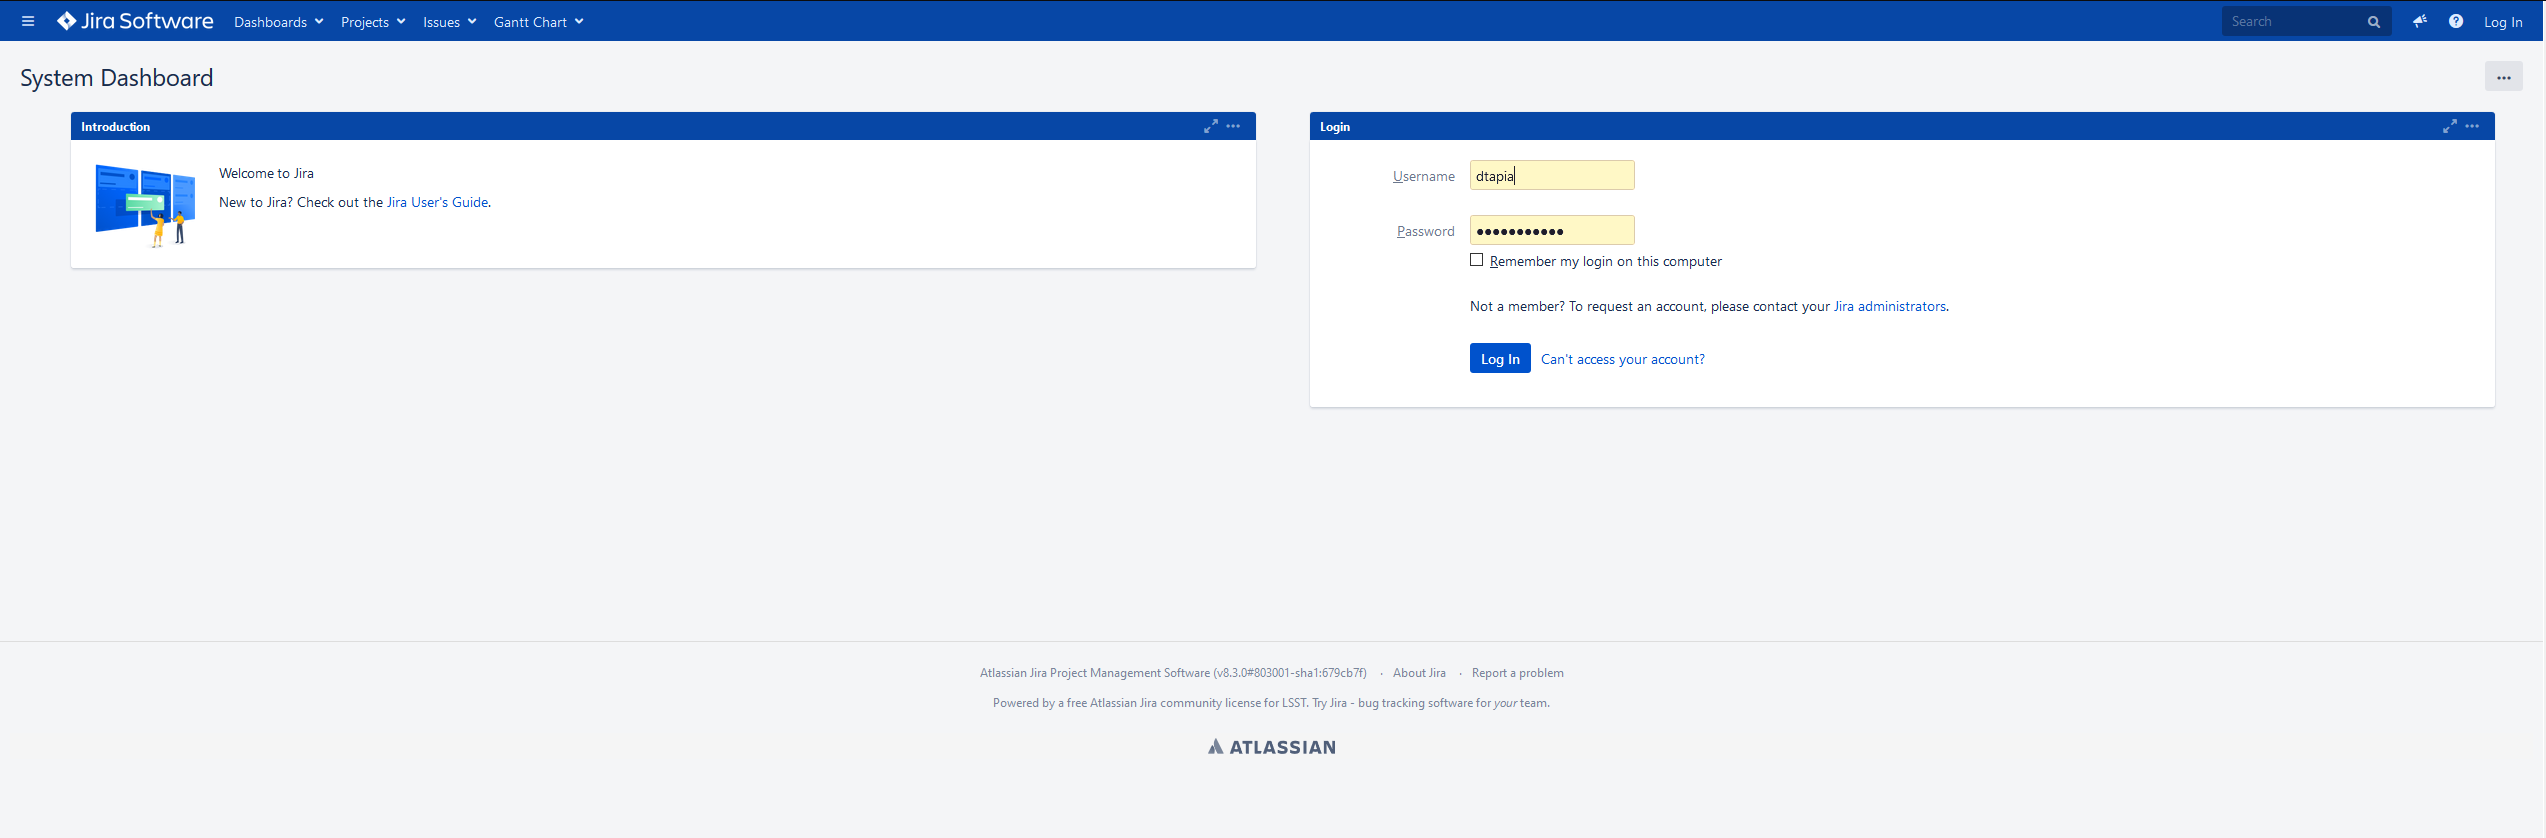
\includegraphics[width=12cm]{Images/example1.png}
\end{figure}

\vspace{5 mm}

Once logged in the user will be prompted with the following windows if not similar. Before creating the ticket,  it is required for the user to check that he is in the proper dashboard for this particular case the IT Support Dashboard

\vspace{5 mm}

\begin{figure}
  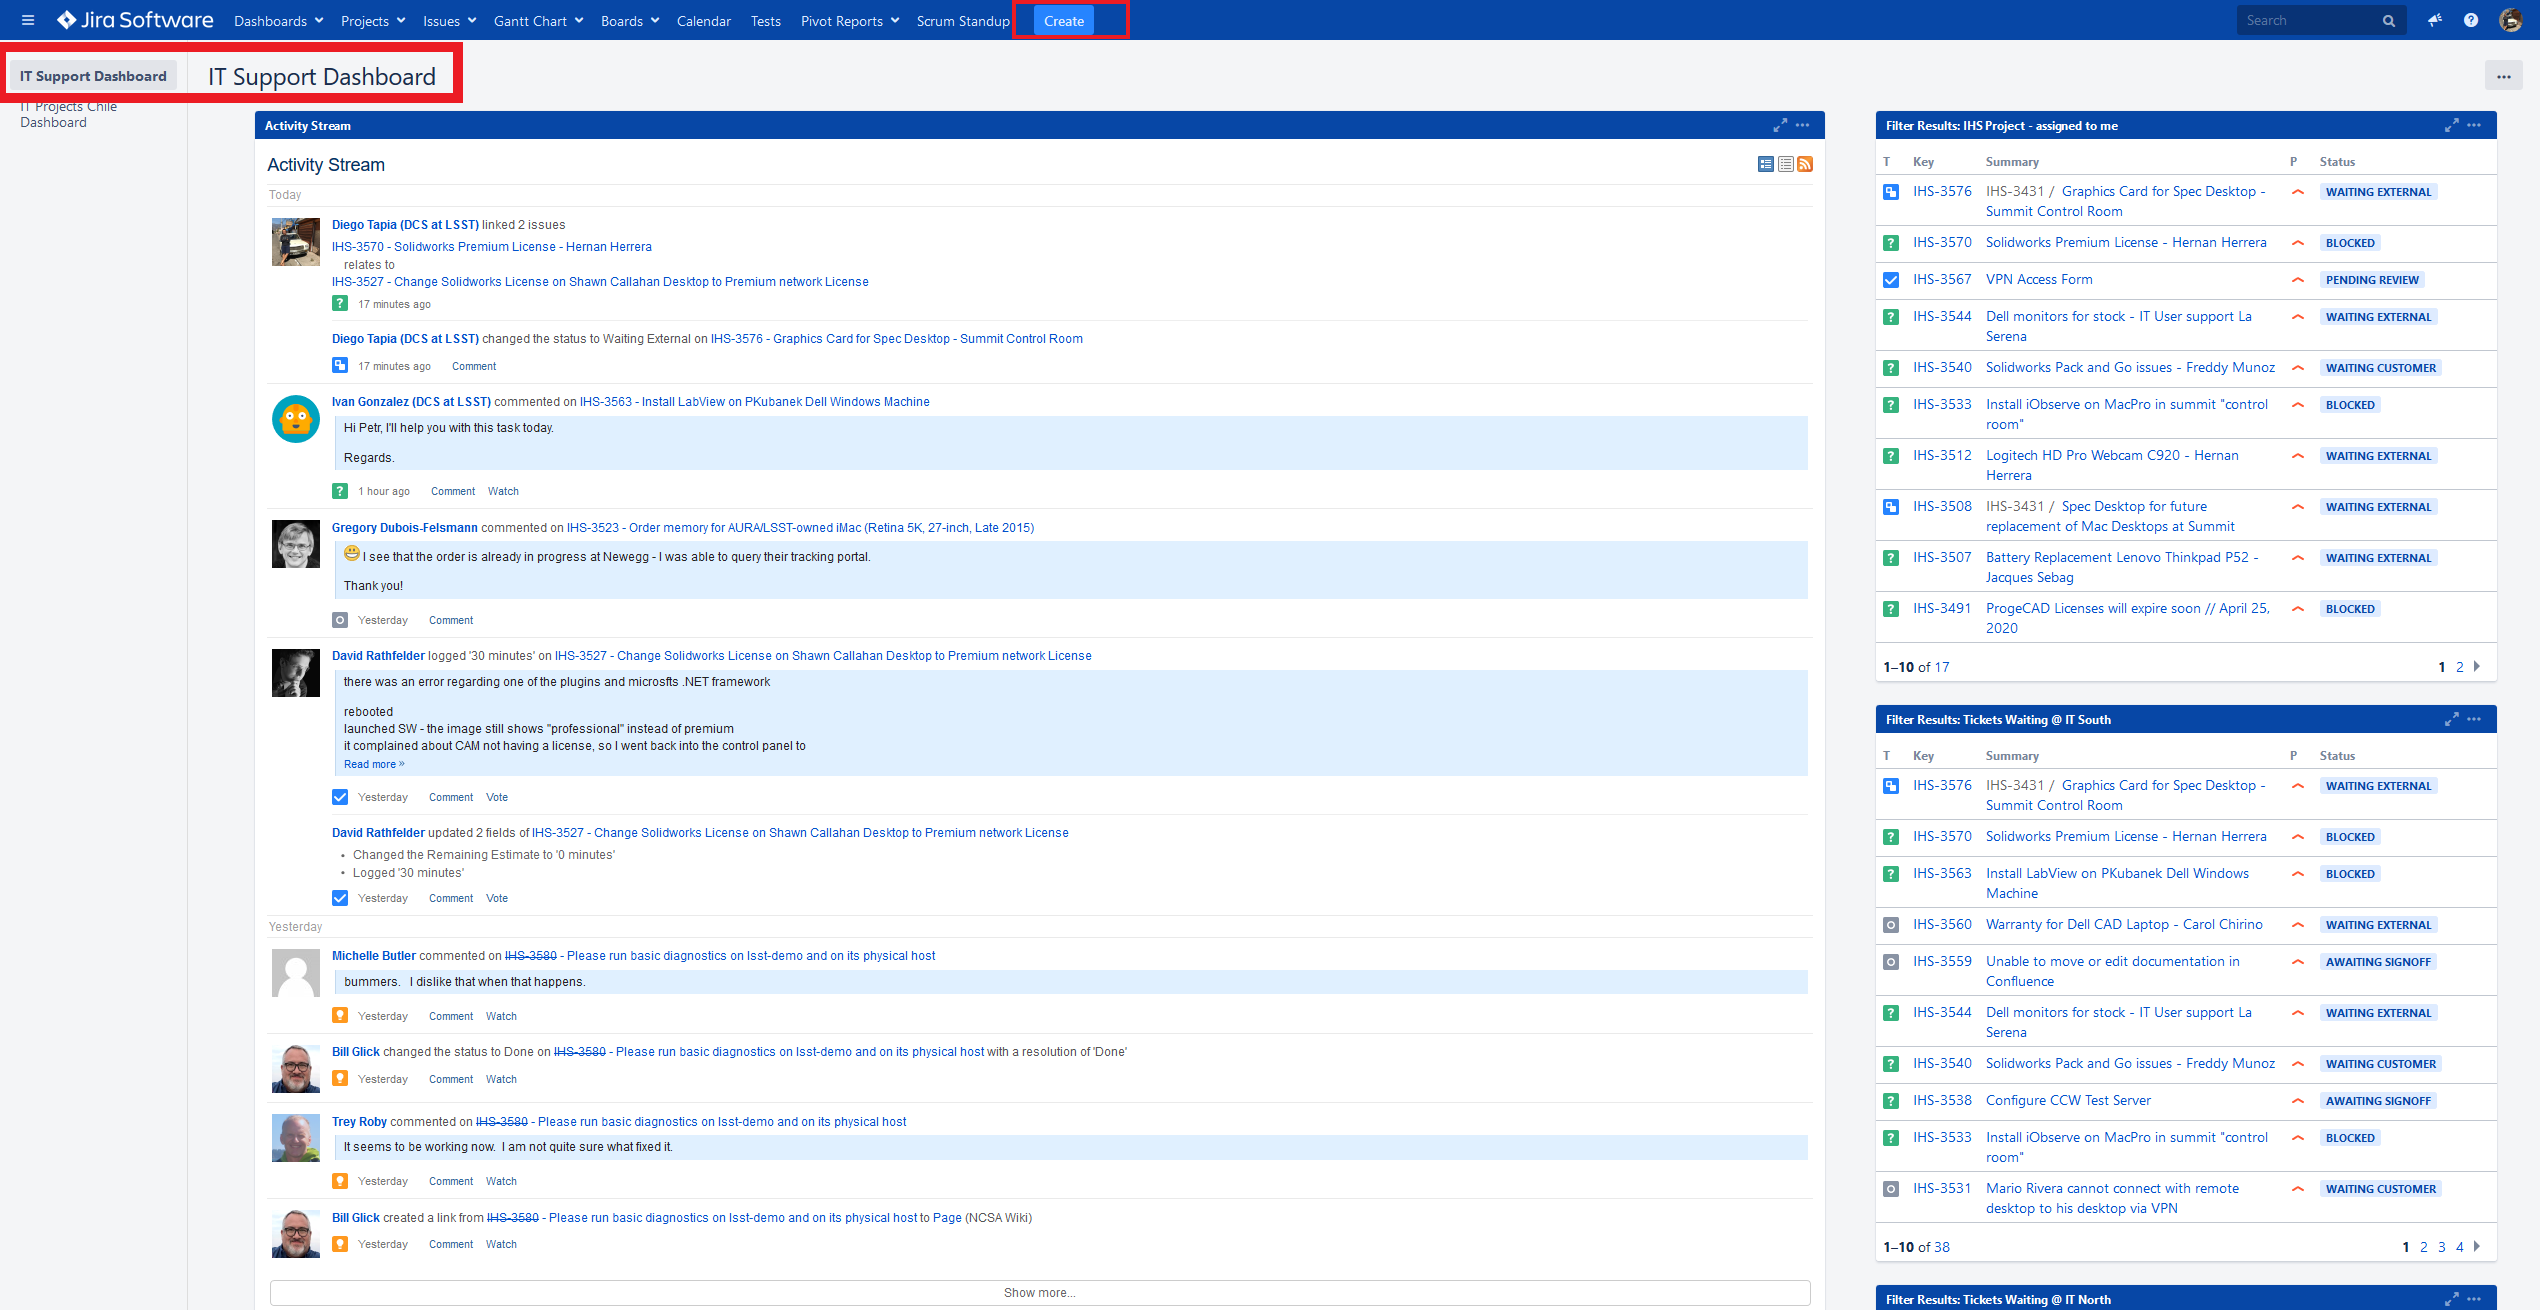
\includegraphics[width=12cm]{Images/example2.png}
\end{figure}

\vspace{40 mm}

On the ticket creation window fill out the template using the information provided below:

\begin{itemize}
  \item Project: IT Helpdesk Support (IHS)
  \item Issue Type: Service Request
  \item Summary: IPA Account Creation / VPN Access - "Insert your name here"
  \item Component: AAA
  \item Description: Please use the template provided below.
\end{itemize}

\vspace{10 mm}

\begin{figure}
  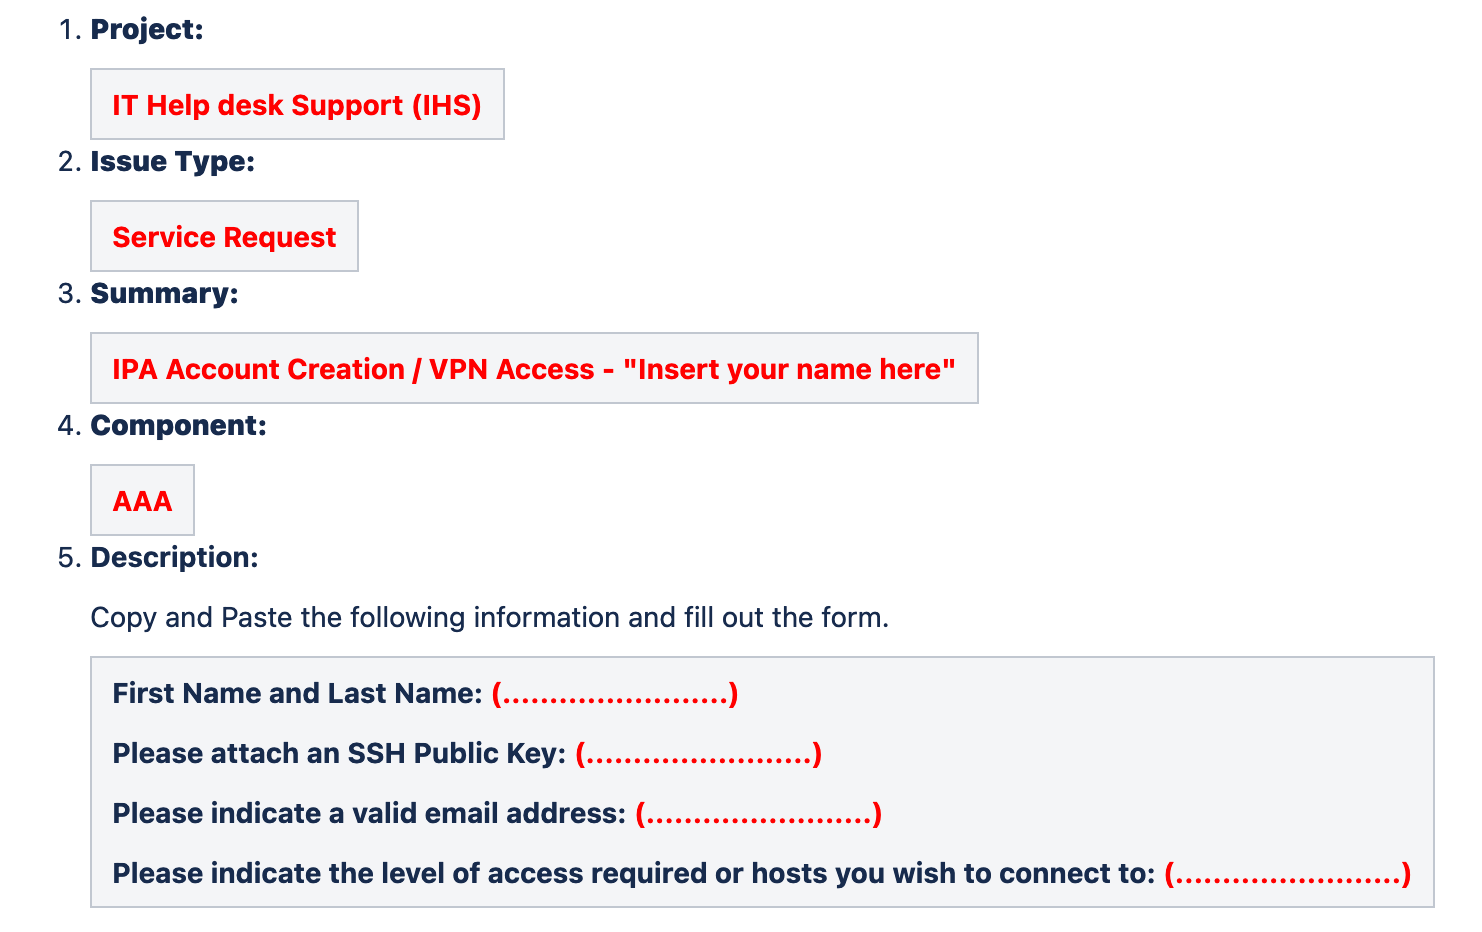
\includegraphics[width=15cm]{Images/example4.png}
\end{figure}

\newpage

Once all the information is filled out, select the Create option located at the bottom to create the ticket inside IHS IT Support Dashboard.

\vspace{10 mm}

\begin{figure}
  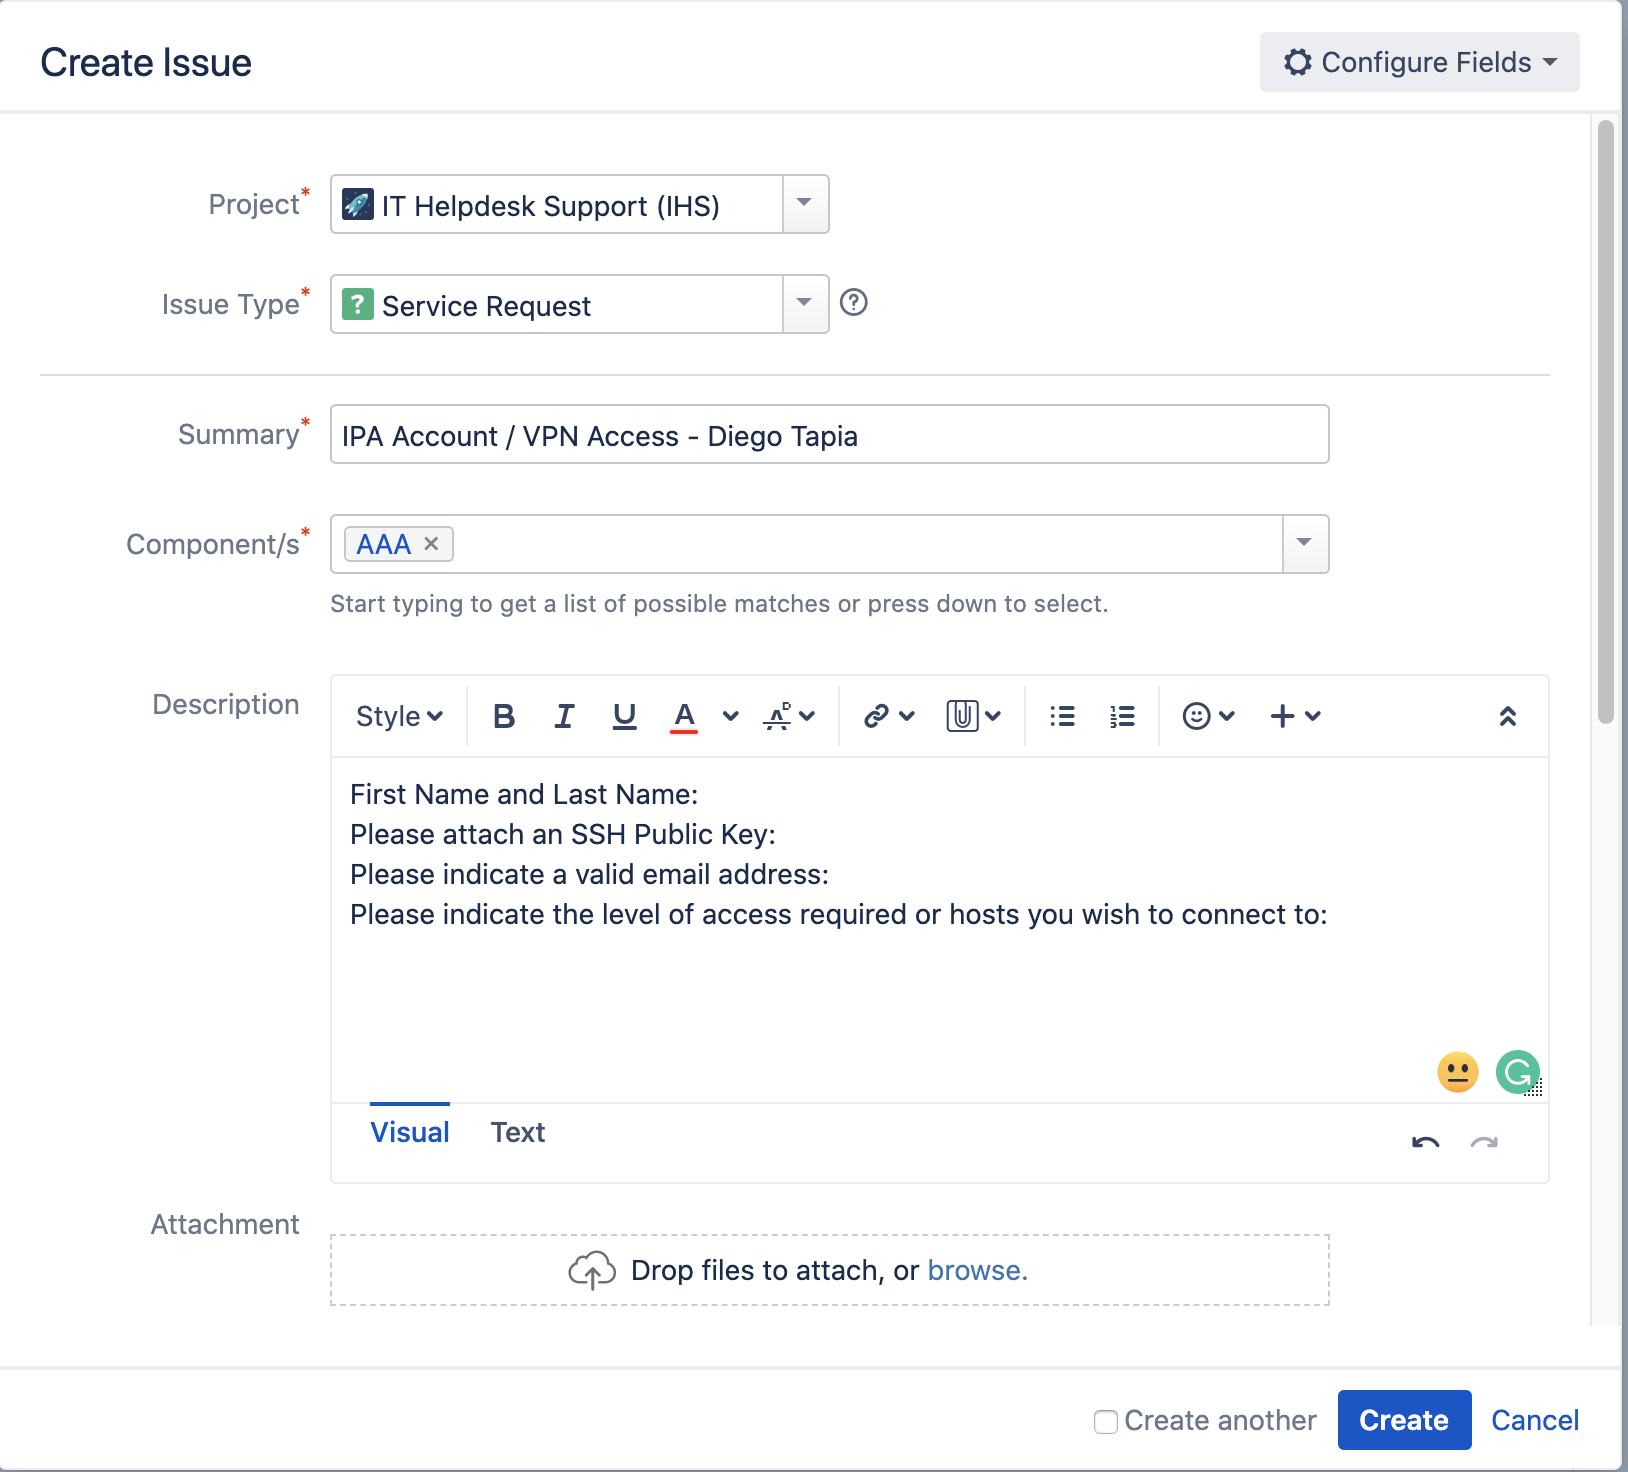
\includegraphics[width=13cm]{Images/example3.png}
\end{figure}

\vspace{10 mm}
IT User support will receive the request and will proceed with the account creation process. Once the account has been created and the services have been provisioned IT Support will be in contact with you via email to provide you with the account credentials and services you've been granted access too along with the website where you can change your temporary password.

If you have any questions or concerns regarding the services provisioned please contact IT User Support at rubinobs-it-las@lsst.org

\subsection{Rubin Server Authentication}
\label{sec:SSH}

All  Rubin  Observatory’s  servers  are  set  to  authenticate  through  FreeIPA  and  Asymmetric Cryptography through  Secure  Shell  (ssh),  and all other  mechanisms  are  blocked.  This  means,  all  local accountsand password authentication are not allowed, so once the servers are admitted to IT’s network and infrastructure, all previous local accounts, passwords, permissions, users and groups IDs (uid and gid).

When  a  new user  arrives,  or  a  user  that  does  not  yet  have  credentials, it  is  requested  to  create  a  RIC (Request for IPA Credentials) following the instructions above. 

Then,  comes  an important part of the process: setting and creation of the Asymmetric Cryptography, also known as public-key cryptography.

\begin{figure}
  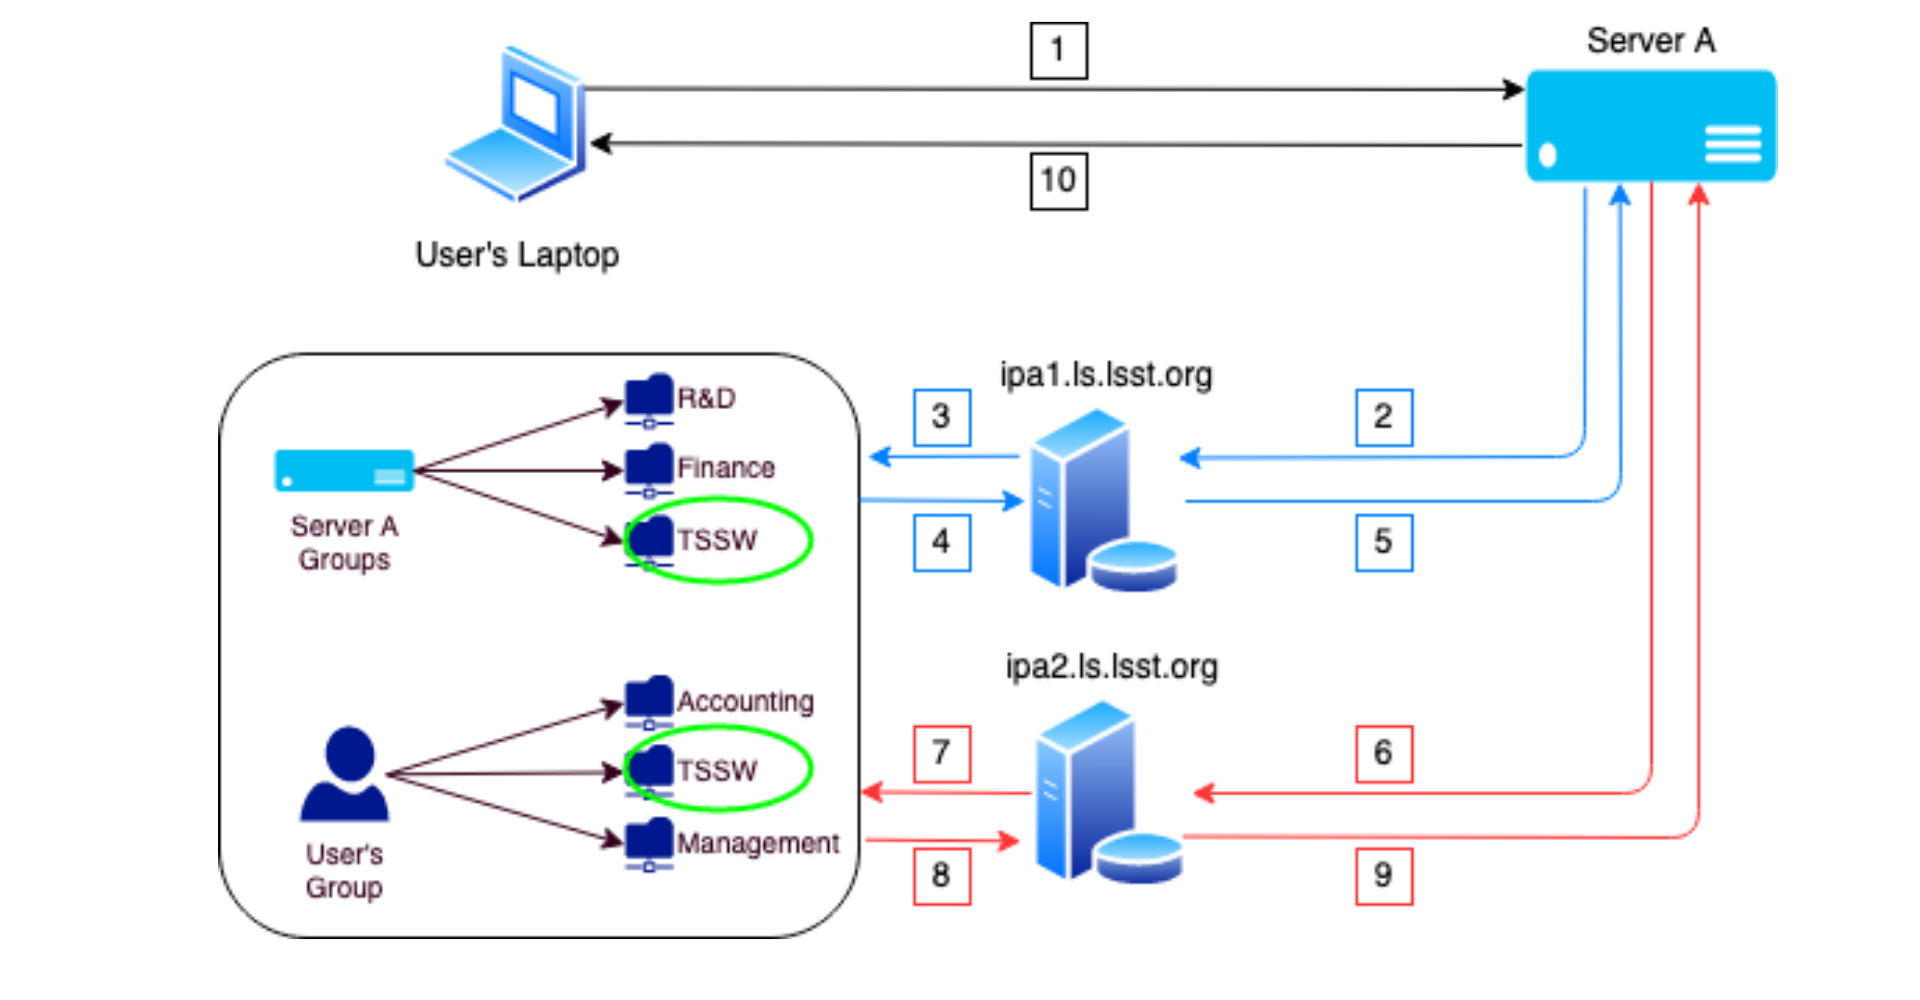
\includegraphics[width=13cm]{Images/example5.png}
\end{figure}

(1) The user presents its private ssh-key, (2) If the primary IPA Server is reachable (ipa1.ls.lsst.org), the
Rubin’s Server (Server A) presents the user’s private key to ipa1, (3) The IPA Server checks against the
common database(among all replicas) if the users exists and matches the private against the stored public
key; if the user exists, it also checks if the group who it belongs has sufficient privileges to access, (4) The 
Server fetches the Database information, (5) The IPA Server either grants or denied access to the User’s
Laptop to Server A, (10) The permission granted/denied is send to the User’s Laptop.
If the Primary IPA Server isn’t reachable after timeout, it does the same operation over the failover (red)
Server, following path 6 -> 7 -> 8 -> 9 instead of 2 -> 3 -> 4 -> 5.

\subsubsection{SSH Keys Creation}
\label{sec:SSH:}

Depending on your OS, is the instructions you will need to follow:

\subsubsection{Linux and MacOS}
\label{sec:SSH}

First, log into your local machine, then search and open a terminal window. Once there:

\begin{figure}
  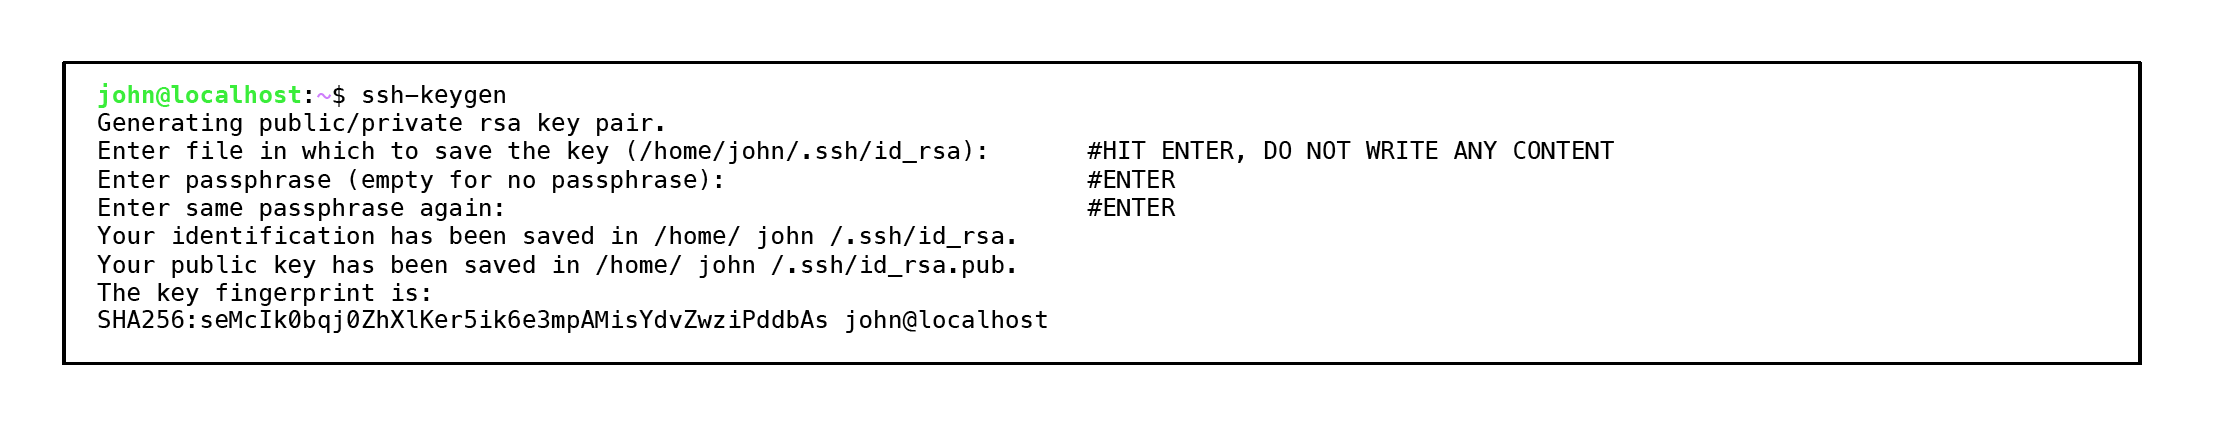
\includegraphics[width=13cm]{Images/example6.png}
\end{figure}

If the John, already has a pair of private/public keys – and for personal reasons don’t want to reuse them –
you can set a new pair by changing the name of the keys and adding a config file, so that the local ssh agent
includes that key as well:

\begin{figure}
  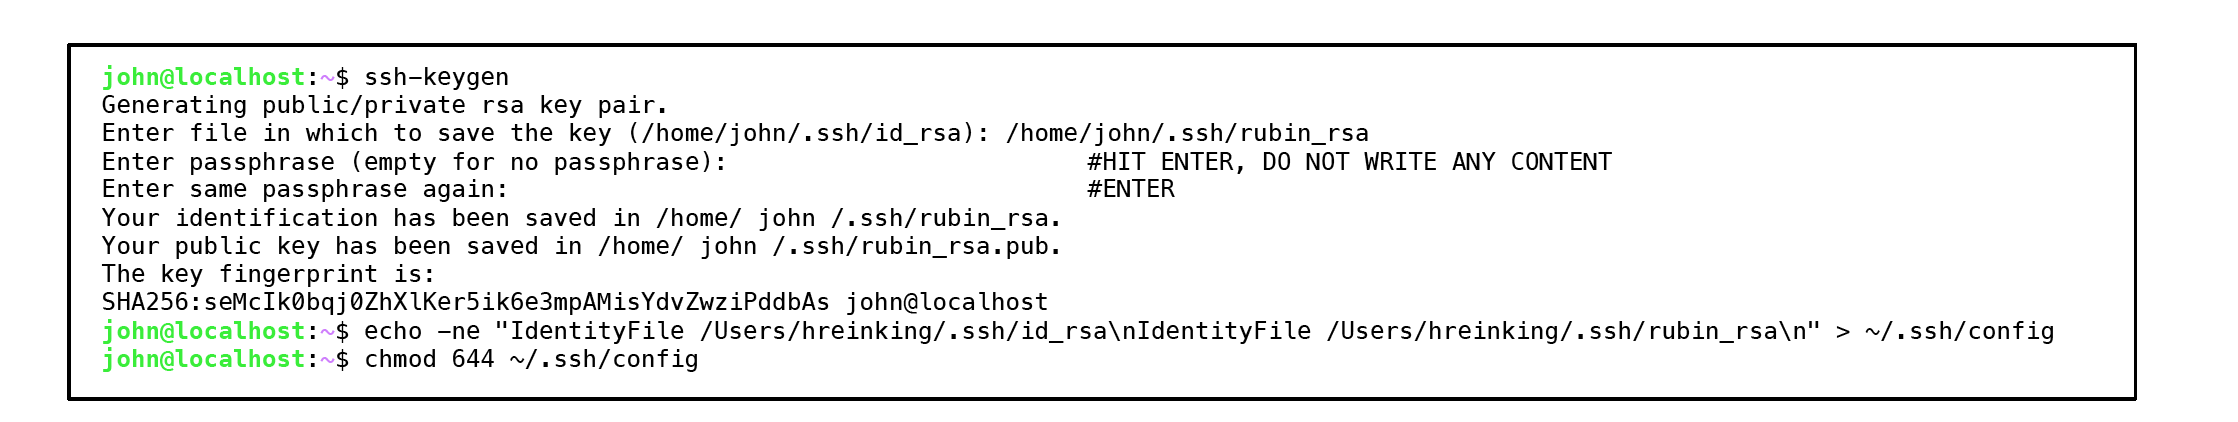
\includegraphics[width=13cm]{Images/example7.png}
\end{figure}

The id_rsa file contains your private key, which by no reason must be shared or known by another person; this will not only compromise the integrity of the server, but also related user’s data, account access, etc. On the other hand, the id_rsa.pub contains the public key, which is intended to share and be publicly known.

\newpage
\subsubsection{Windows OS}
\label{sec:SSH}

Windows does not natively have a native ssh mechanism. There are several third-party applications,
designed to satisfy such need, but we are going to use PuTTY9, which is an Open-Source software SSH and
Telnet client \href{https://the.earth.li/~sgtatham/putty/latest/w64/putty-64bit-0.74-installer.msi}{Putty Client}.


Once PuTTY is installed, we will use a complementary tool (already installed along with putty) called
PuTTYgen (you can open it by typing it into Windows Search box):

\vspace{5 mm}

\begin{figure}
  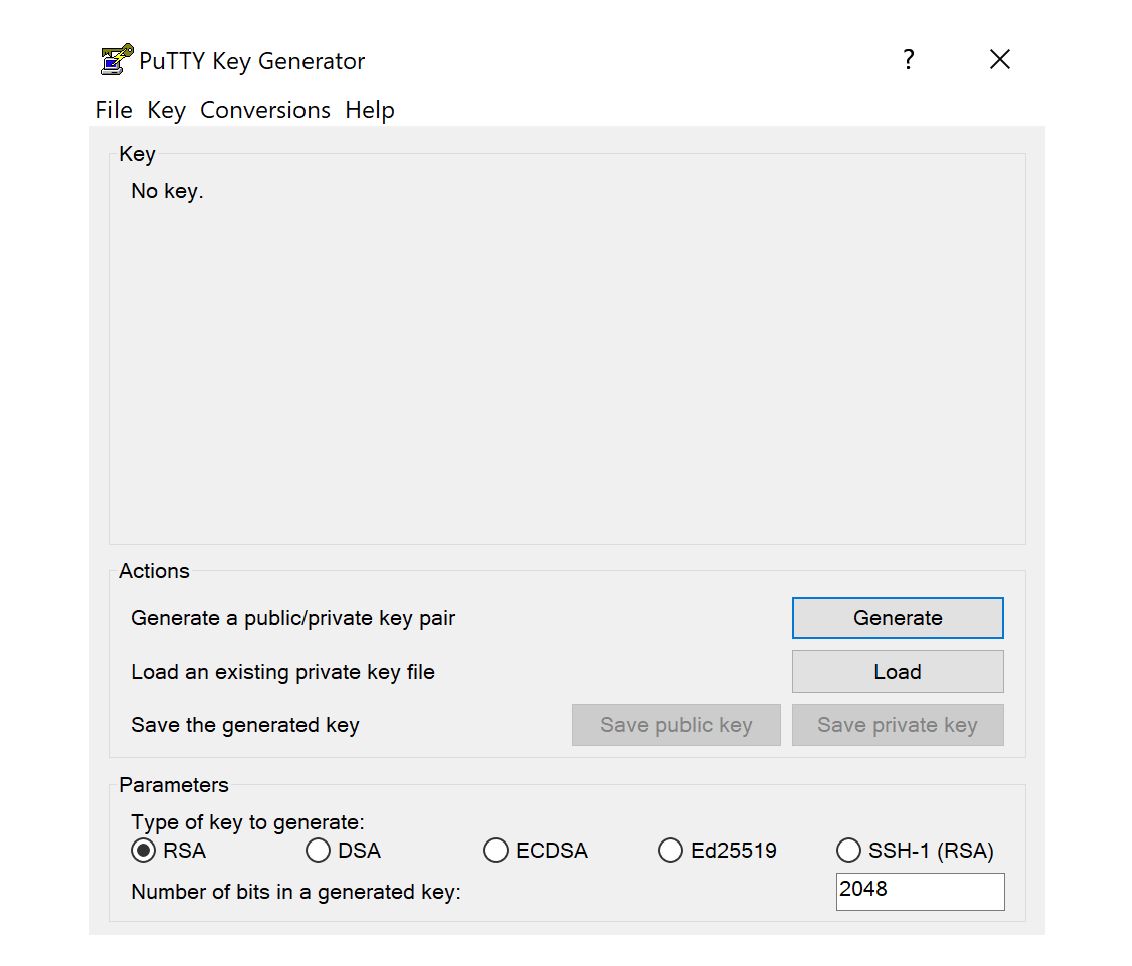
\includegraphics[width=13cm]{Images/example8.png}
\end{figure}

\newpage

Click on generate:

\begin{figure}
  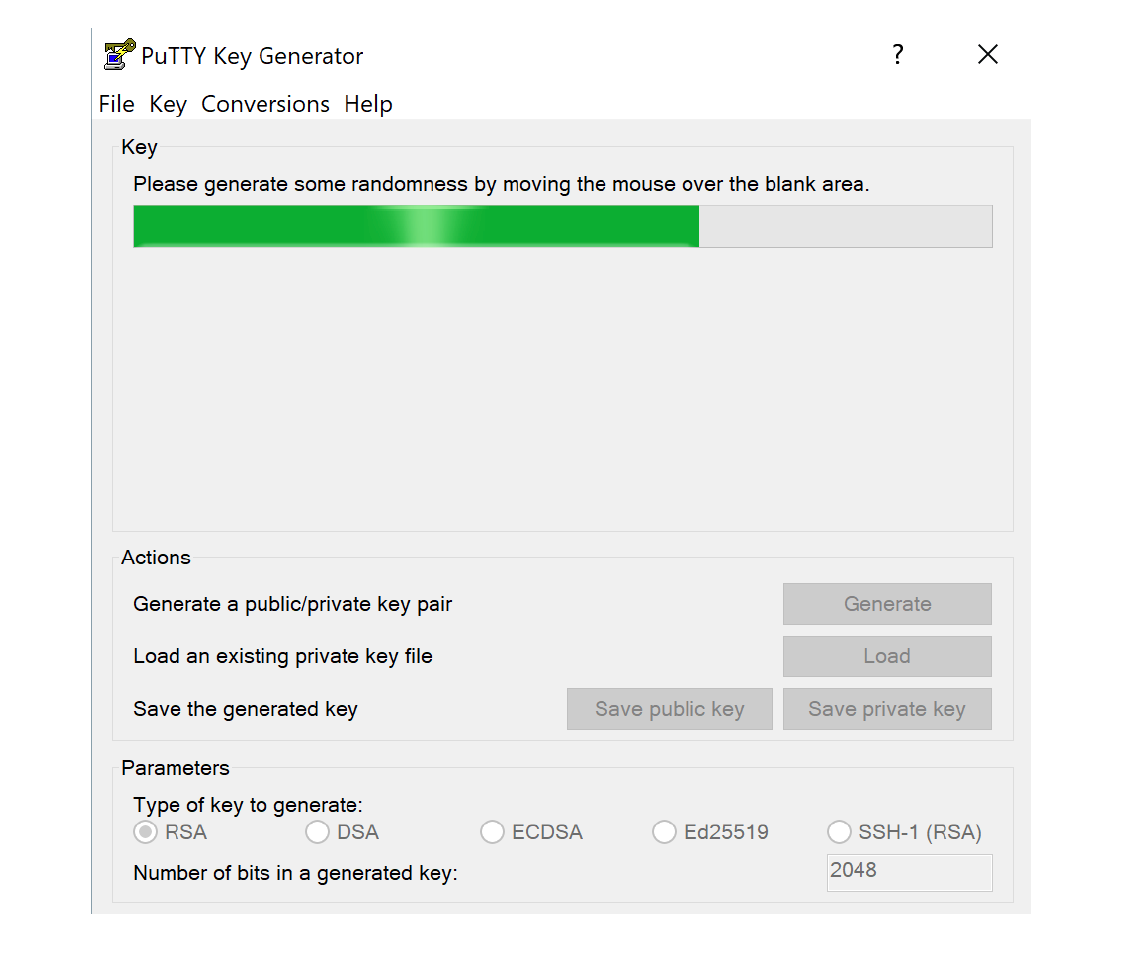
\includegraphics[width=13cm]{Images/example9.png}
\end{figure}

In order to create a random key, you must move the mouse over the surface, so the progress bar moves.
\newpage

Once concluded, you should see something like:

\begin{figure}
  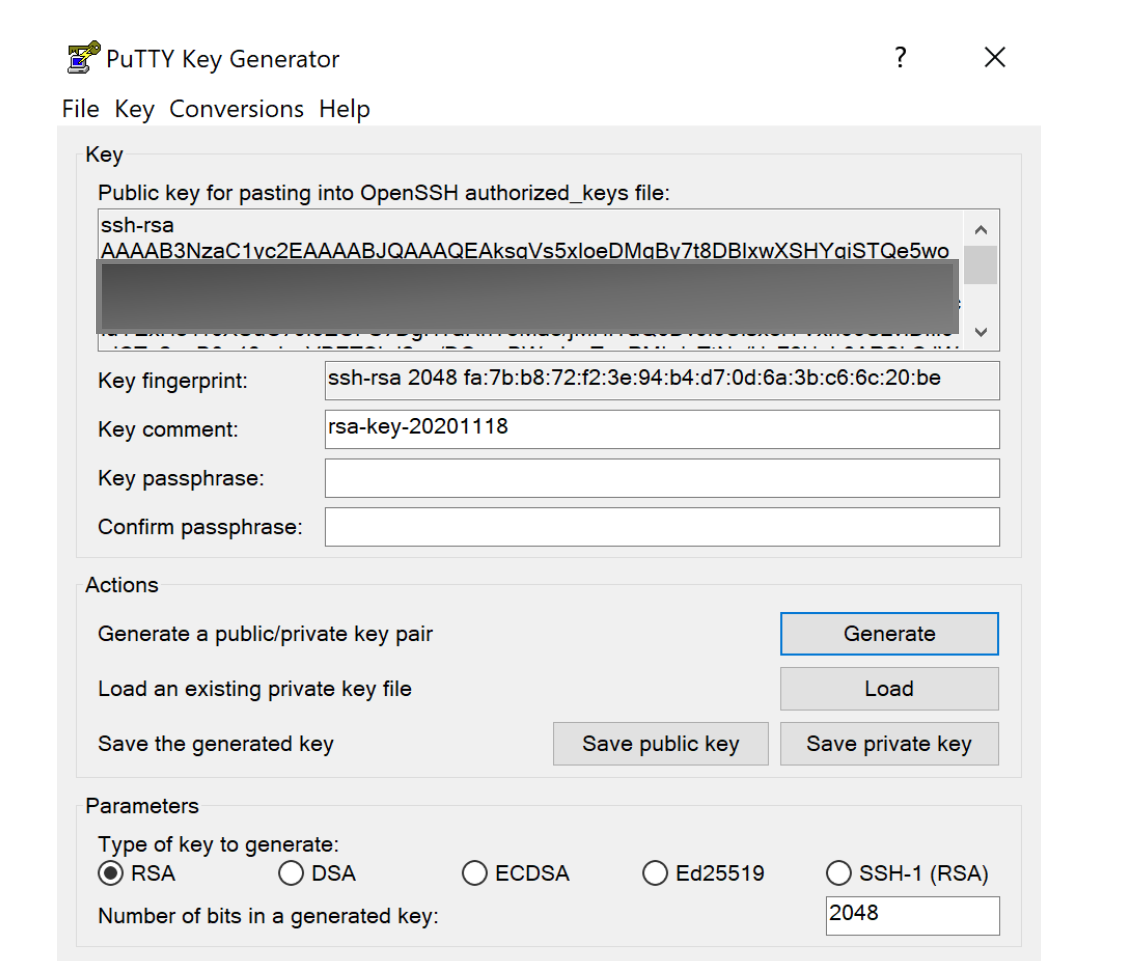
\includegraphics[width=13cm]{Images/example10.png}
\end{figure}

\vspace{5 mm}
Now, save both keys into a well-known location. It is recommended (but not needed) to create a folder
named “ssh” in the user’s home directory, so when asked, you can easily find your keys in
“/Users/<username>/ssh/”.

\newpage

\subsubsection{Add Public Key Into IPA}

The IPA infrastructure is composed of a master server and several replicas, meaning that it does
not matter in which one you modified your personal data, it will be propagated over the rest of the nodes.

\vspace{5 mm}

The IPA Topology (Image below) is designed in such way, that in the worst-case scenario, at least one source
of authentication will remain.

\begin{figure}
  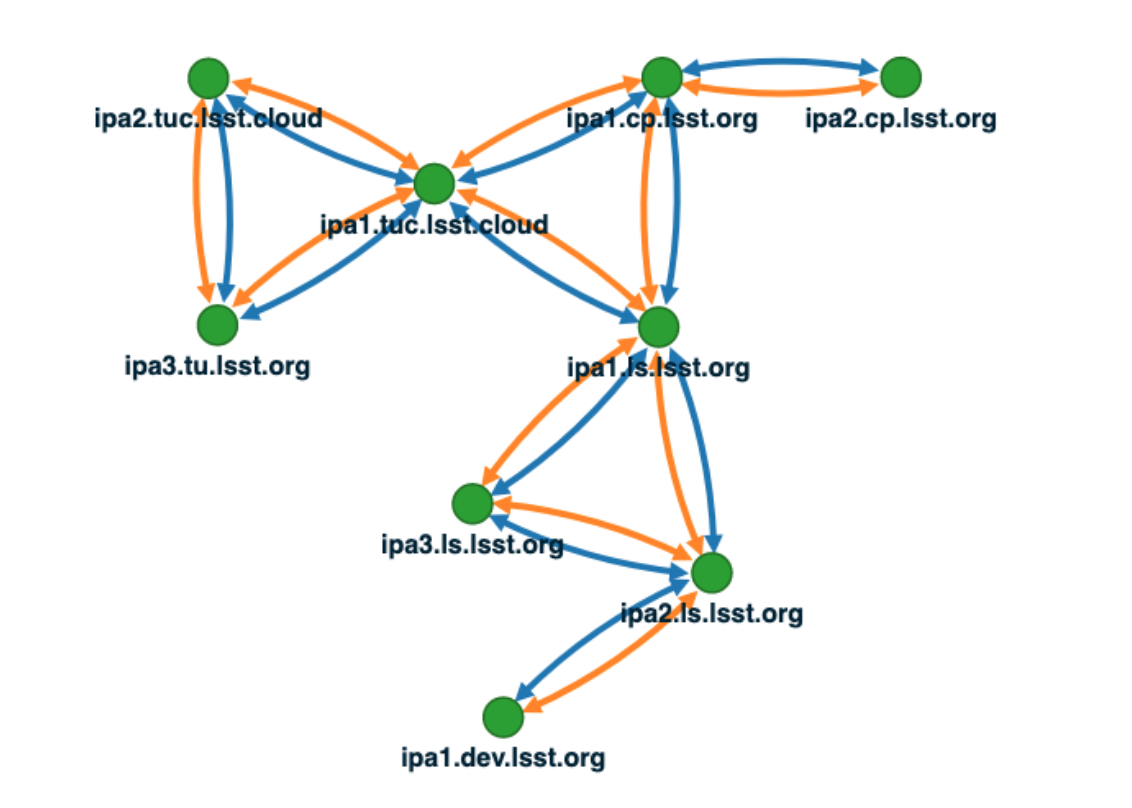
\includegraphics[width=13cm]{Images/example11.png}
\end{figure}

The orange arrows represent the DL (Domain Link), meanwhile the blue arrows the CA (Certificate
Authority). The DL keeps the authenticity of the defined domain – i.e. server.local – and the CA is the
responsible of emitting and signing the hosts certificates, to validate their authenticity.

\vspace{5 mm}
\newpage

In order to add your public key into IPA, you must access through any of the http frontends, from either
the replicas or master. Bear in mind that you must be either inside the network or connected through VPN.
Let’s use the BDC (Base Data Center) replica: open a web-browser and navigate to \href{https://ipa1.ls.lsst.org}{IPA Website}.
You should see a welcoming screen:

\begin{figure}
  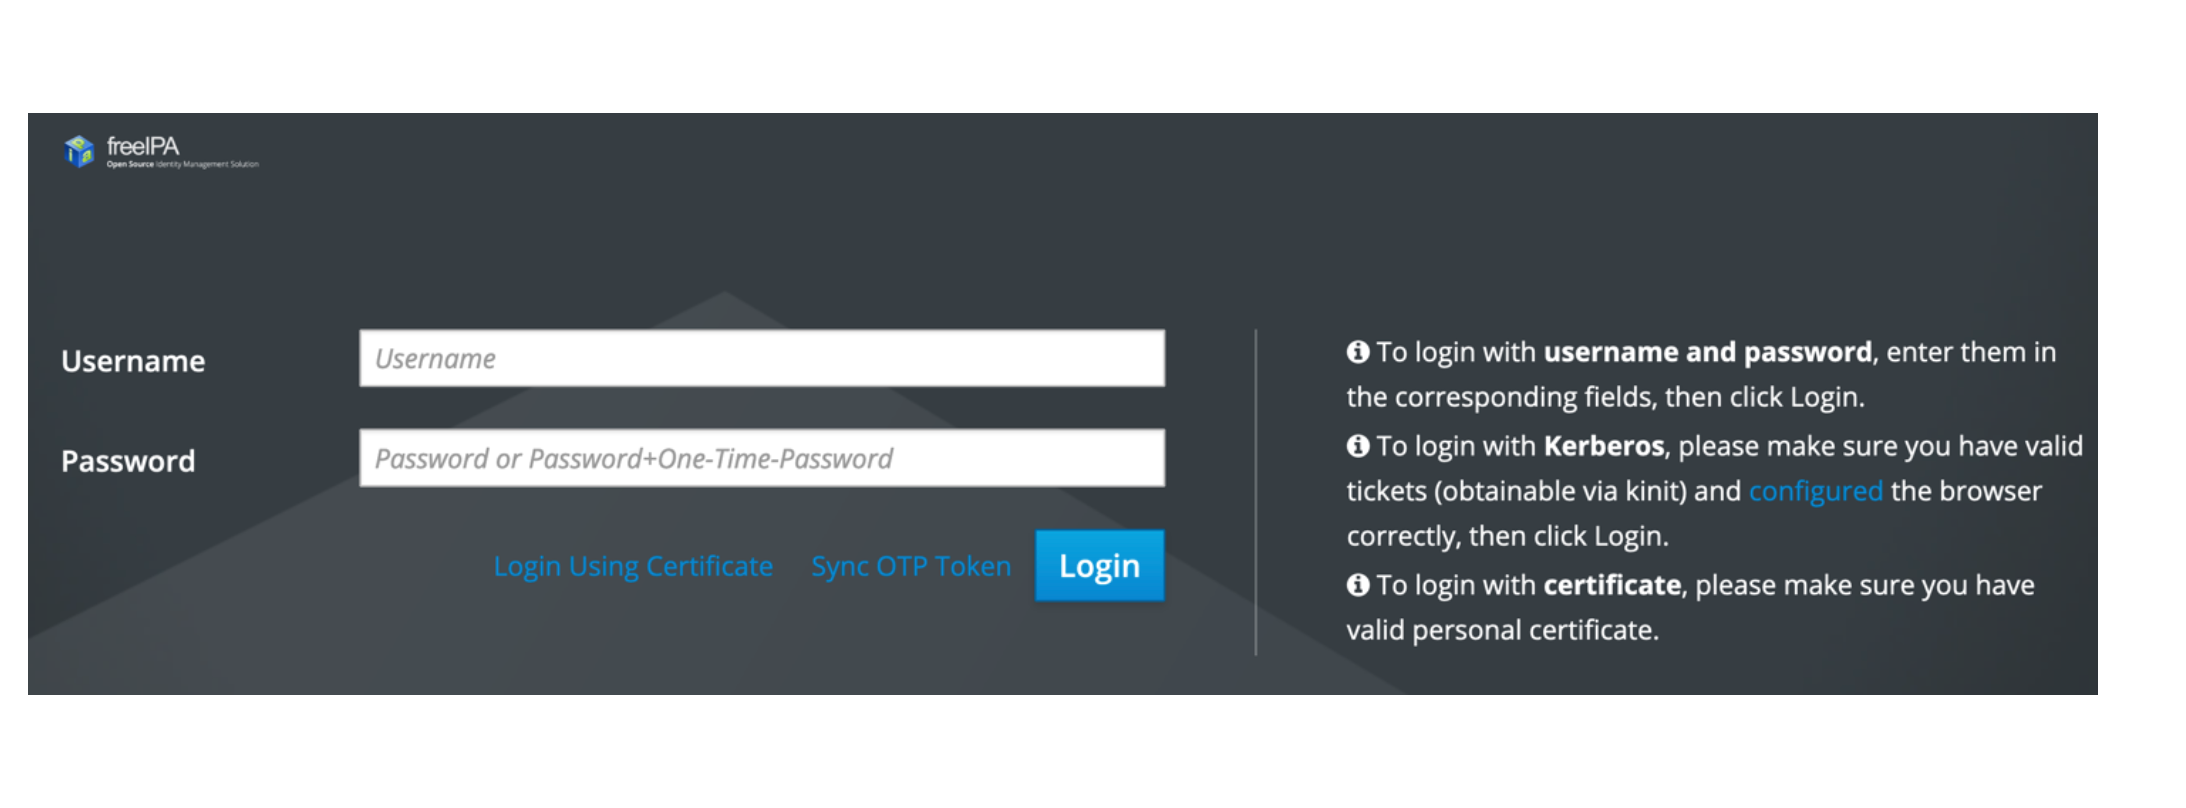
\includegraphics[width=13cm]{Images/example12.png}
\end{figure}


If it’s the first time you log in, the system will force you to change your password (also if it has expired).
Once successfully logged in the platform, (1) in the upper right corner click your username, (2) profile, and
then (3) Add:


\begin{figure}
  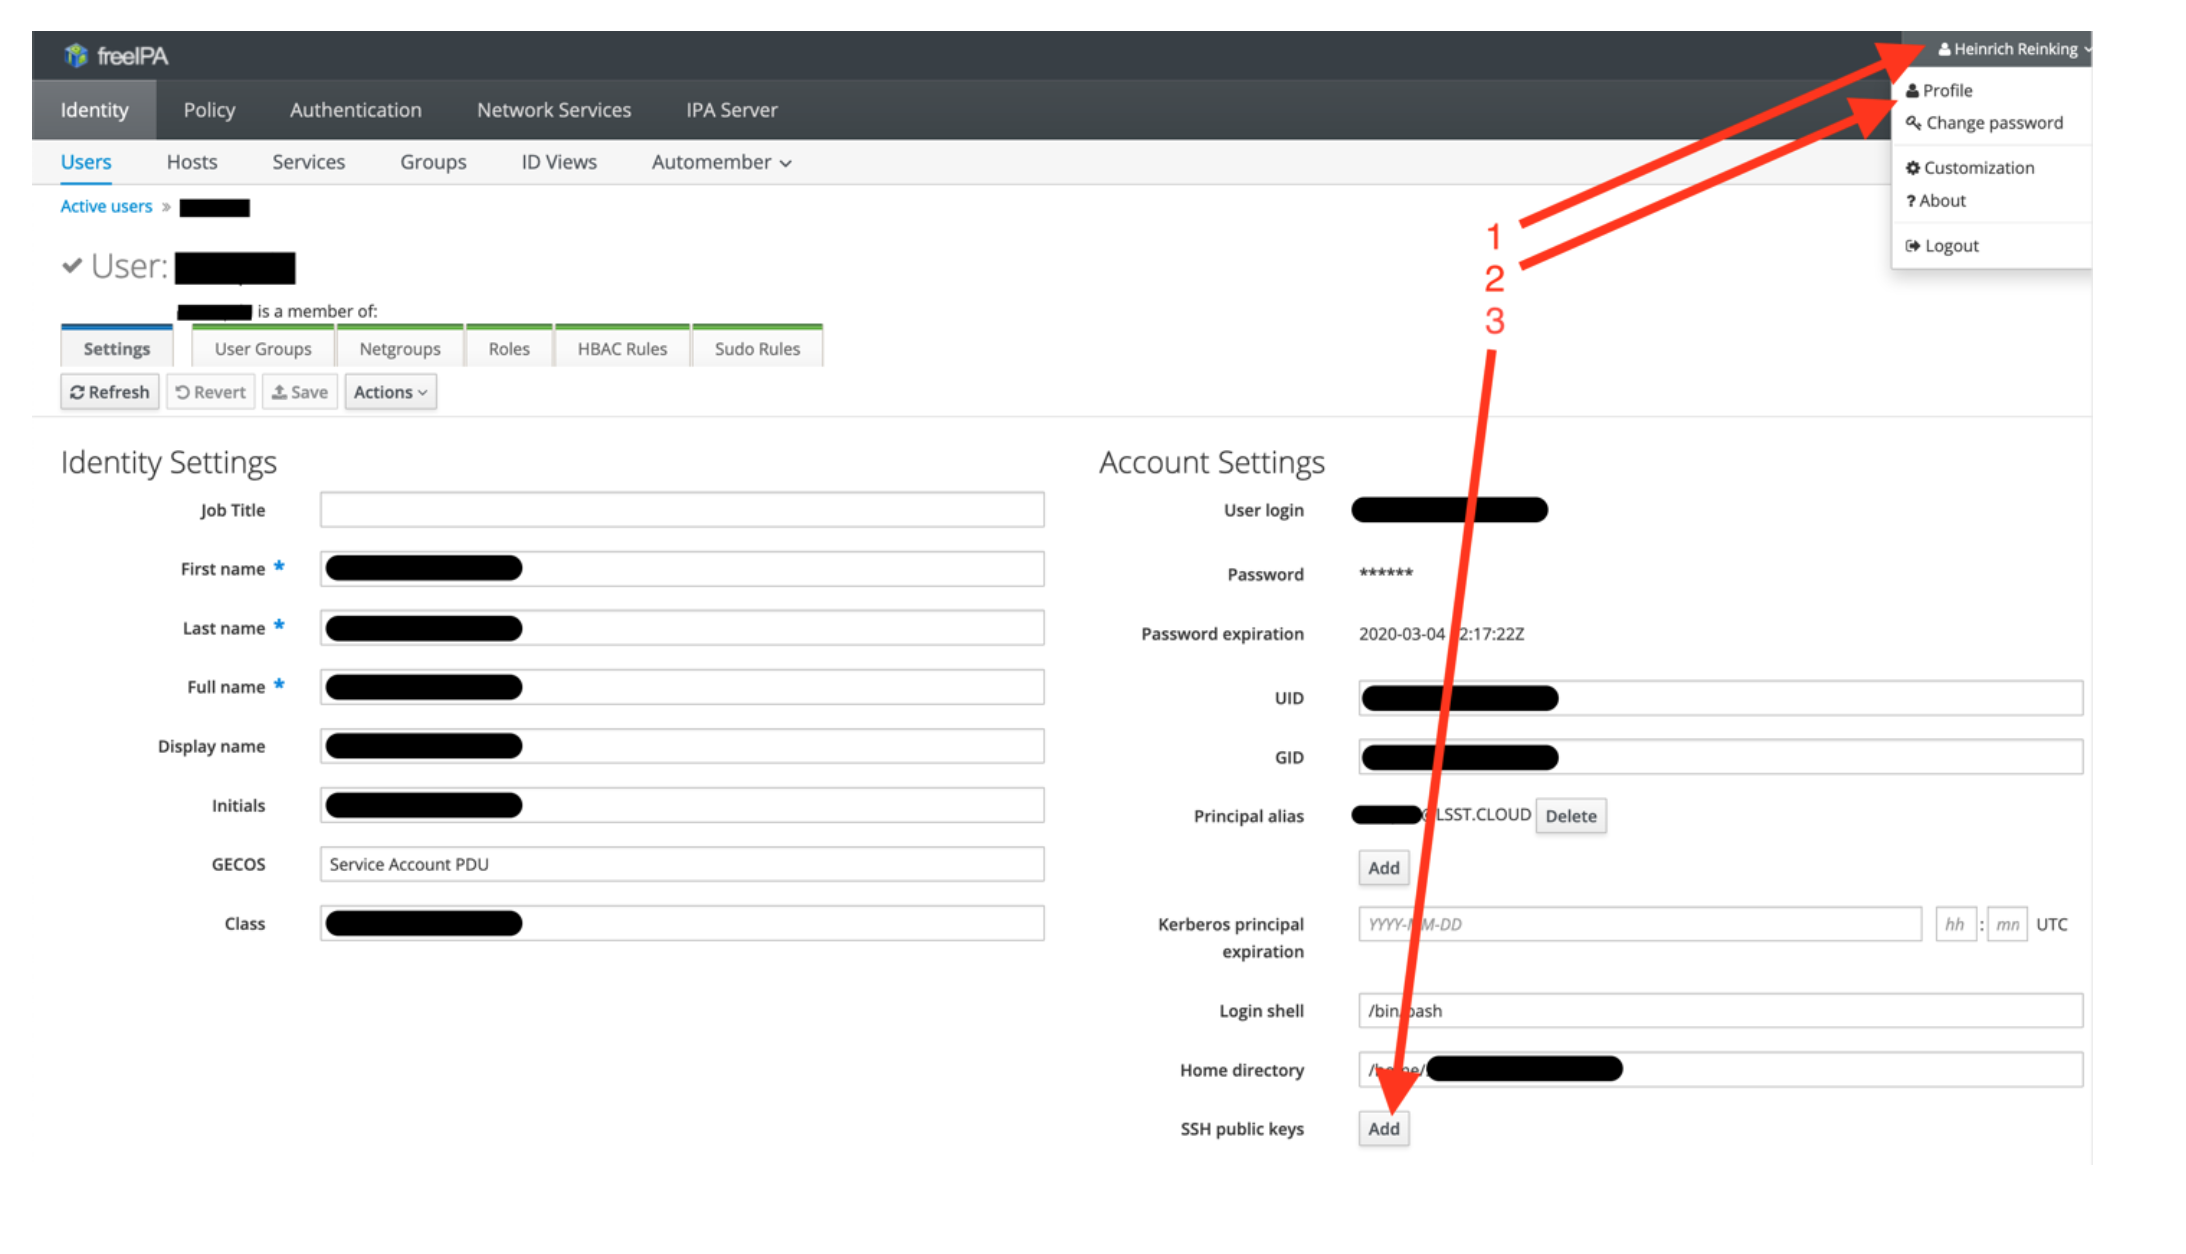
\includegraphics[width=13cm]{Images/example13.png}
\end{figure}

\newpage

A pop-up window will appear, in which you must paste your public key:

\begin{figure}
  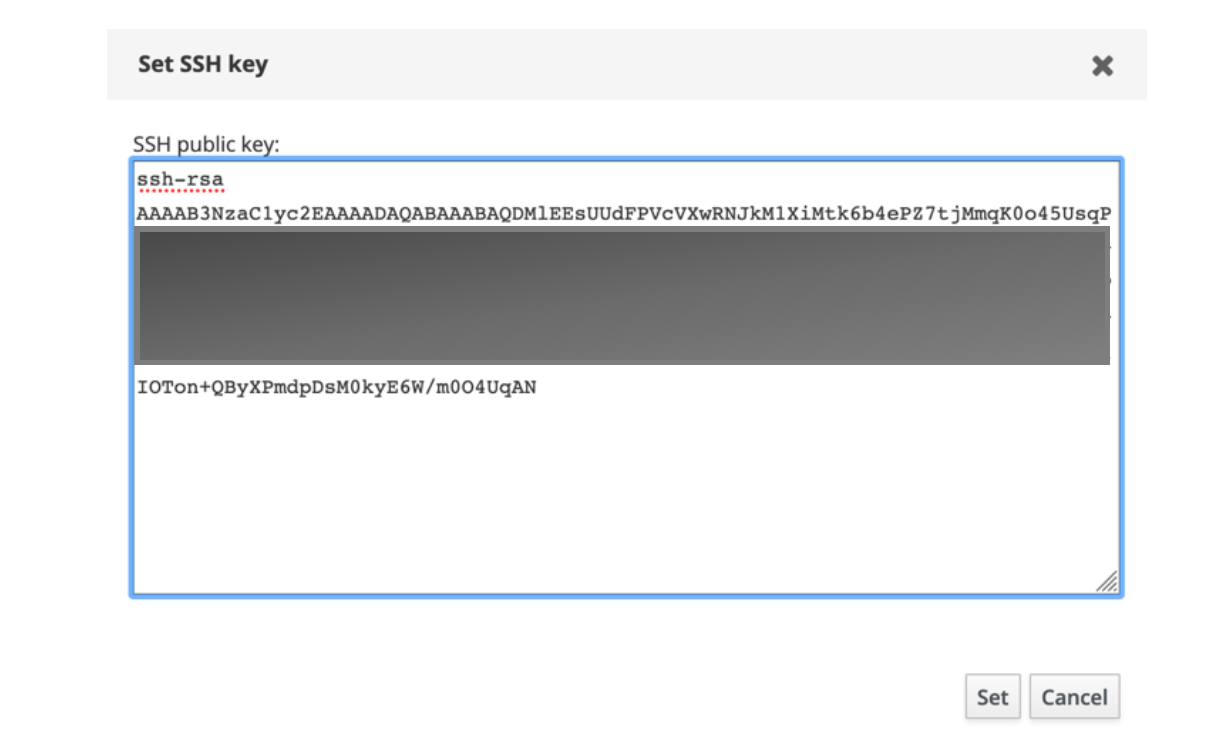
\includegraphics[width=13cm]{Images/example14.png}
\end{figure}

If you are importing a key generated with PuTTY, must use only the selected section:

\begin{figure}
  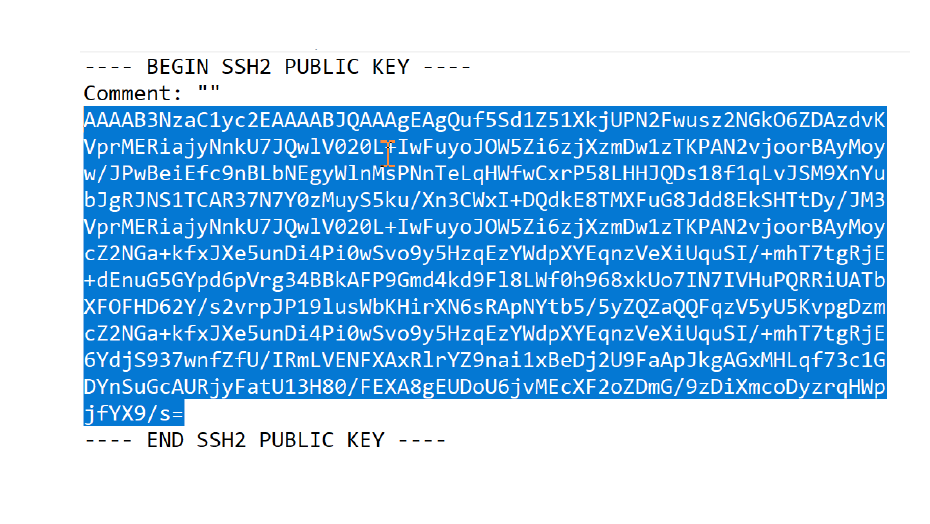
\includegraphics[width=13cm]{Images/example15.png}
\end{figure}

\newpage

If everything was set correctly, click Set, and you will find yourself in the previous window:

\begin{figure}
  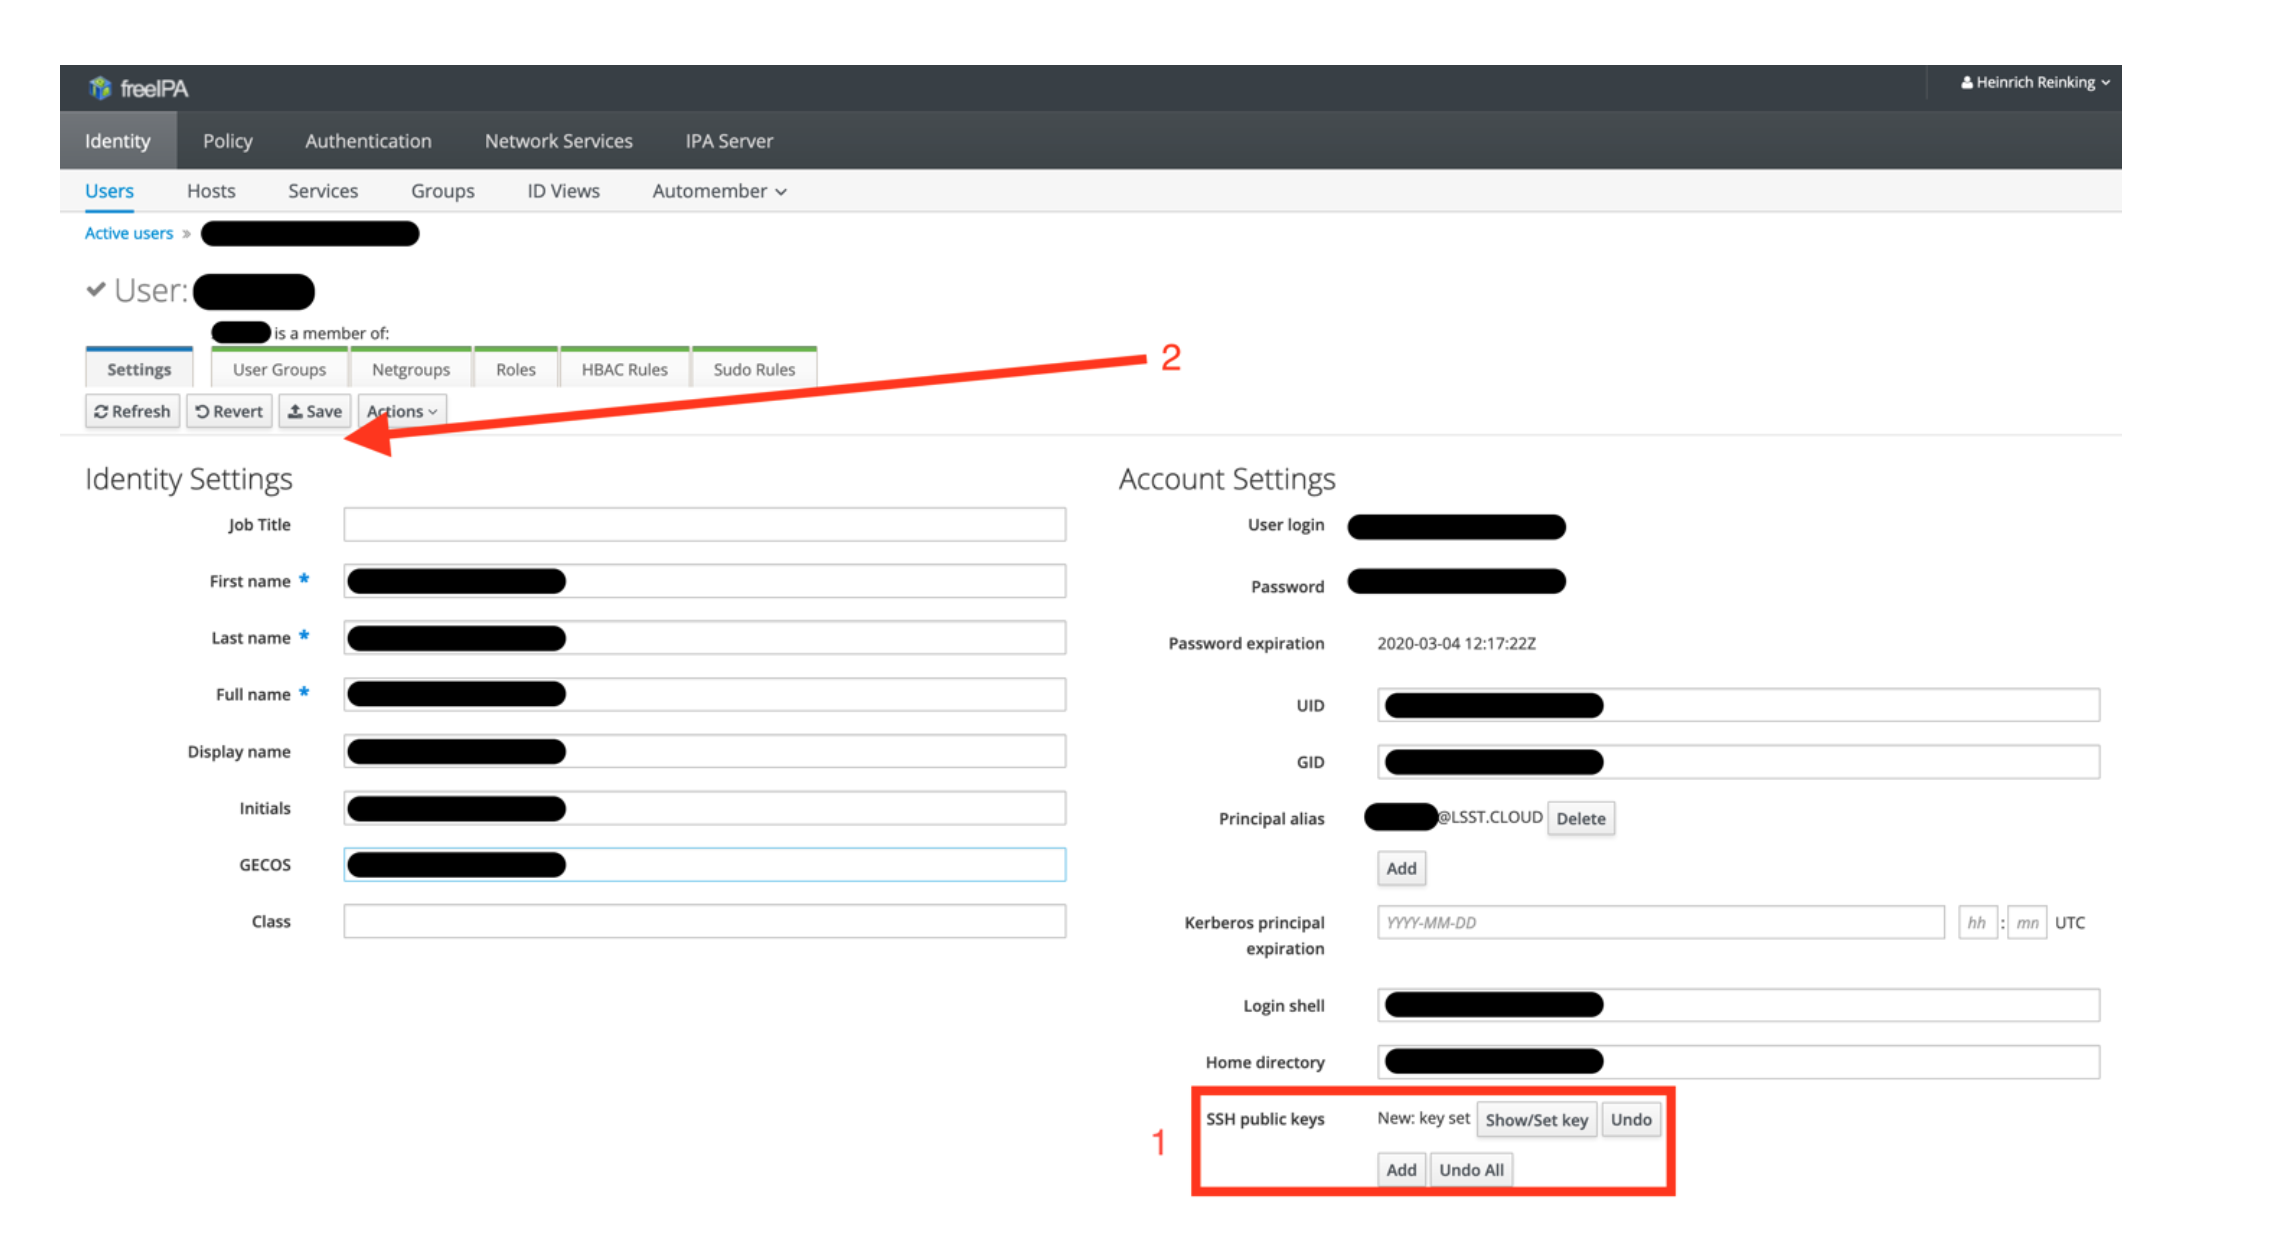
\includegraphics[width=13cm]{Images/example16.png}
\end{figure}

(1) A “New:key set” should now appear and in order for the changes to take place, (2) click on Save.

\newpage

\section{Requesting Domain Credentials}
\label{sec:Domain}

To request Domain Account Credentials, it is required that an Onboarding form is filled out by the manager or supervisor in charge at \href{https://project.lsst.org/onboarding/form}{Onboarding Form}. Once the onboarding form is filled out and submitted with the information requested, IT North will proccess the credentials and will contact the person requesting the access. 

\section{Requesting Nublado Access}
\label{sec:Nublado}

The access to Nublado is controlled by \href{https://github.com}{Github}, hence the user requesting access must have a Github account.

To request access open a DM ticket in Jira including:

\begin{itemize}
  \item Name
  \item Email
  \item Github account
\end{itemize}

A member of the Square team will grant you access. 